\documentclass[c]{beamer}
\usepackage[utf8]{inputenc}
\usepackage{graphicx}
\usepackage{amsfonts}
%\usepackage{fourier}
\usepackage{wasysym}
\usetheme{Warsaw}


\title{Projet Grand Prix}
\author{Hicham Benjelloun}
\institute{ENSICAEN}
\date{14 juin 2013}

\begin{document}

\logo{
\includegraphics[height=15mm]{logo.jpg}}

\begin{frame}
\transdissolve[duration=1]
\titlepage
\end{frame}

\begin{frame}
\transdissolve[duration=1]
  \tableofcontents
\end{frame}


\begin{frame}[label=objectifs]
\transdissolve[duration=1]
\frametitle{Objectifs de base}
\section{Objectifs de base}
Réaliser un pilote :

\begin{enumerate}
\item Qui termine tout type de carte.
\item Qui termine une carte en un nombre quasi optimal de coups.
\item Qui soit robuste.
\end{enumerate}
\end{frame}

\begin{frame}[label=structures]
\transdissolve[duration=1]
\frametitle{Structures de données utilisées}
\section{Structures de données utilisées}
Graphe des états possibles = Tableau 4D de sommets
\end{frame}

\begin{frame}[label=structures1]
\transdissolve[duration=1]
\frametitle{Graphe des états possibles}
\subsection{Graphe des états possibles}
\begin{figure}[!h]
\centering
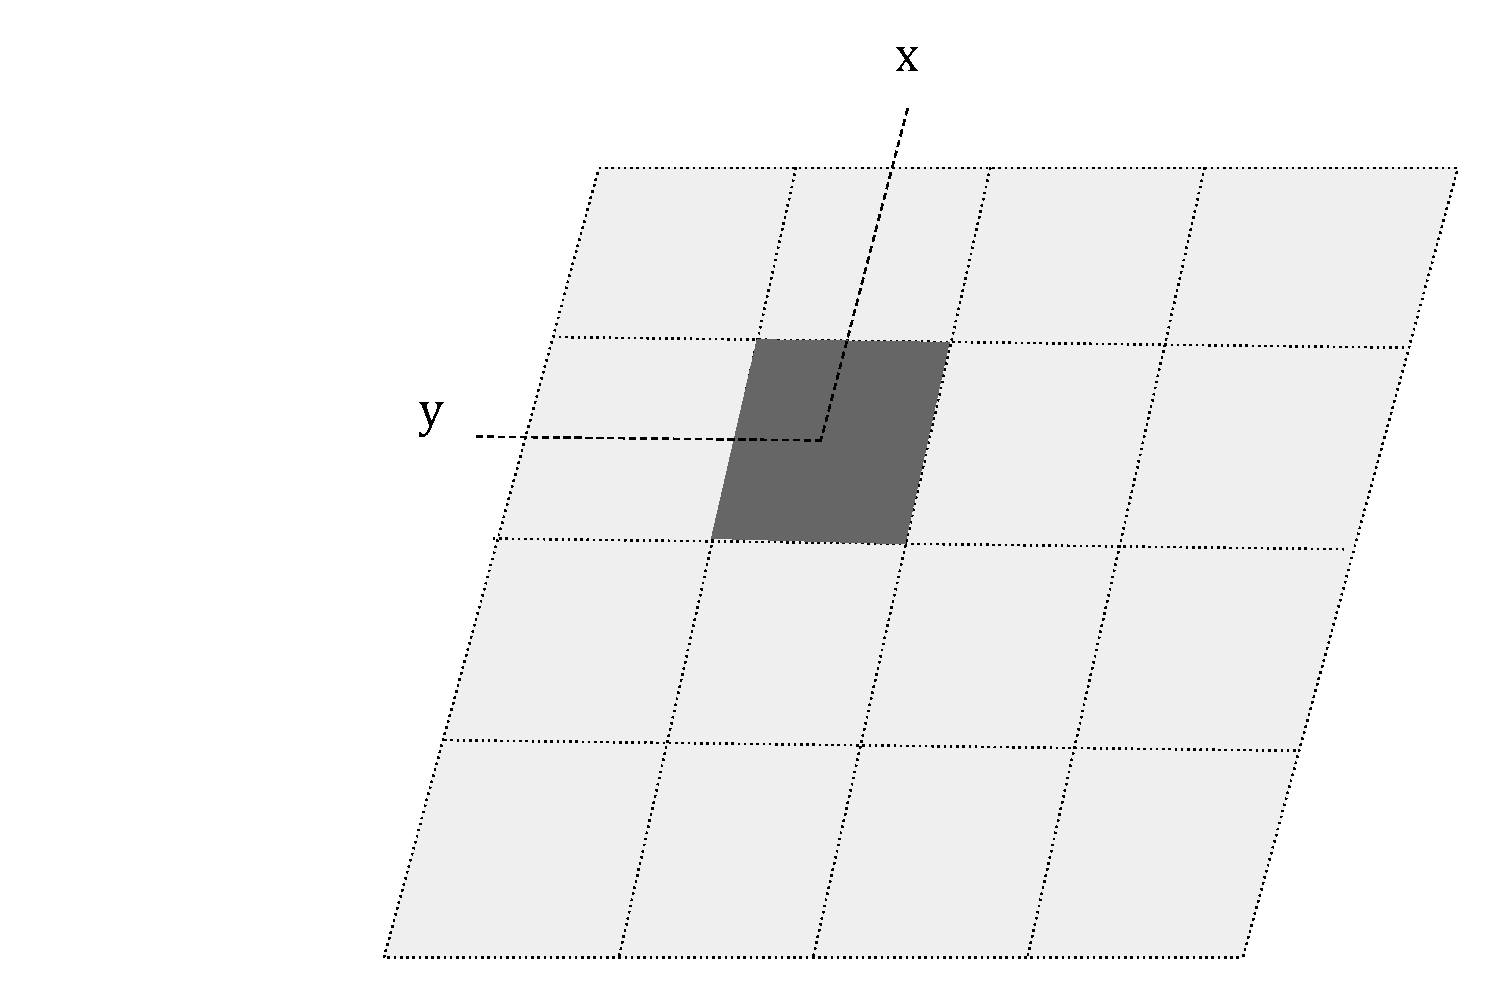
\includegraphics[scale=0.3]{fig/g001.pdf}
\end{figure}
\end{frame}

\begin{frame}[label=structures2]
\transdissolve[duration=1]
\frametitle{Graphe des états possibles}
\begin{figure}[!h]
\centering
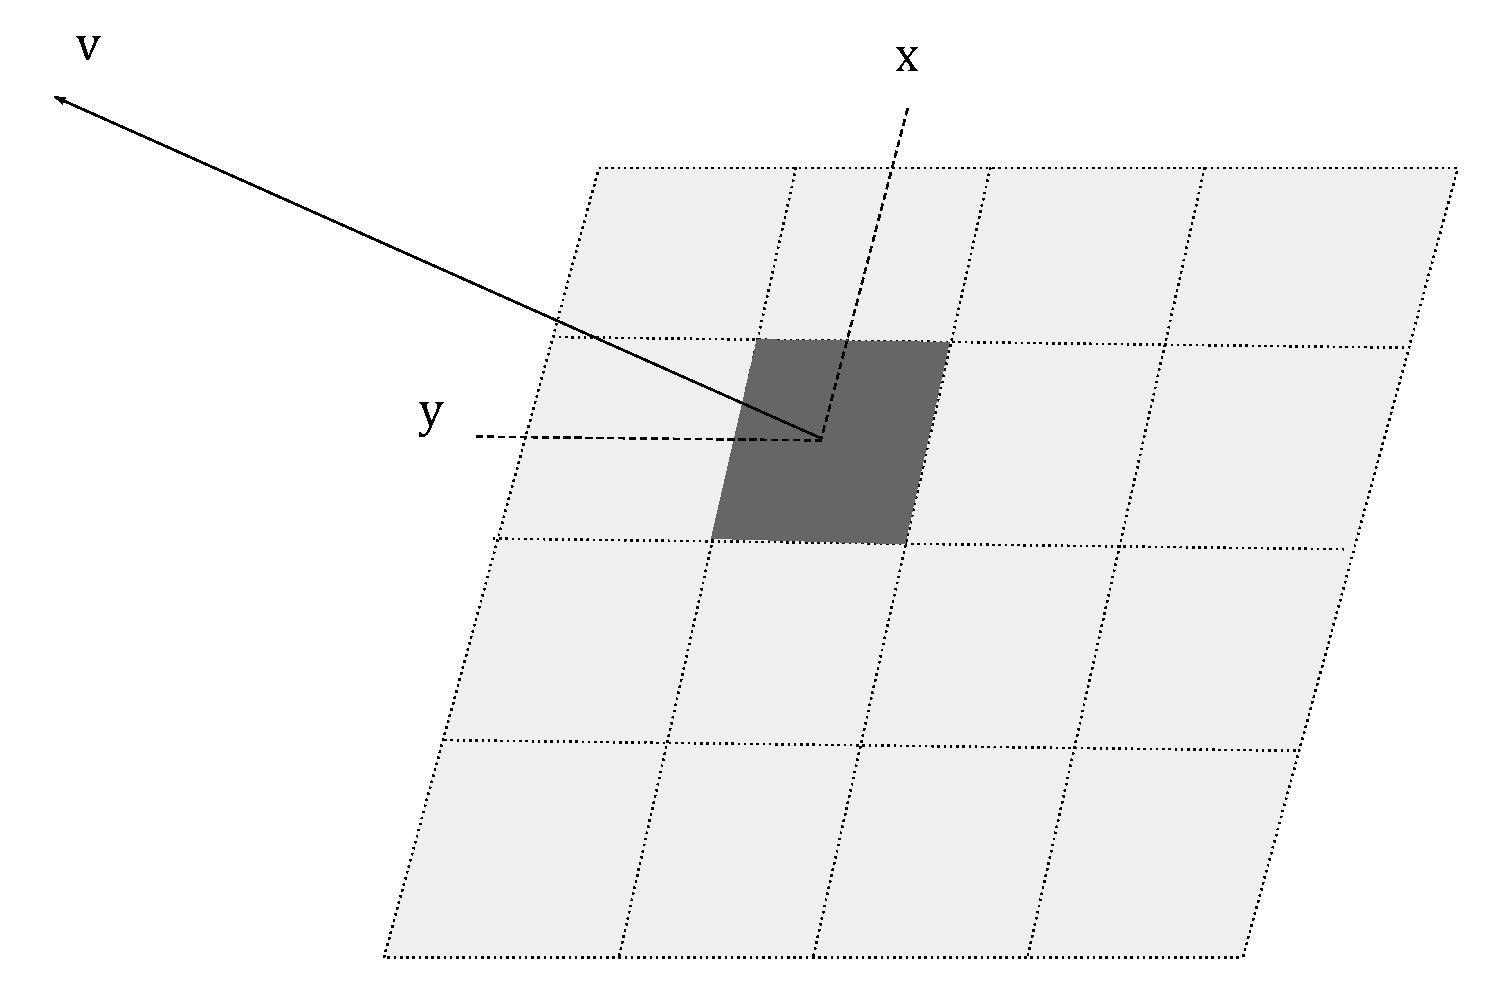
\includegraphics[scale=0.3]{fig/g002.pdf}
\end{figure}
\end{frame}

\begin{frame}[label=structures3]
\transdissolve[duration=1]
\frametitle{Graphe des états possibles}
\begin{figure}[!h]
\centering
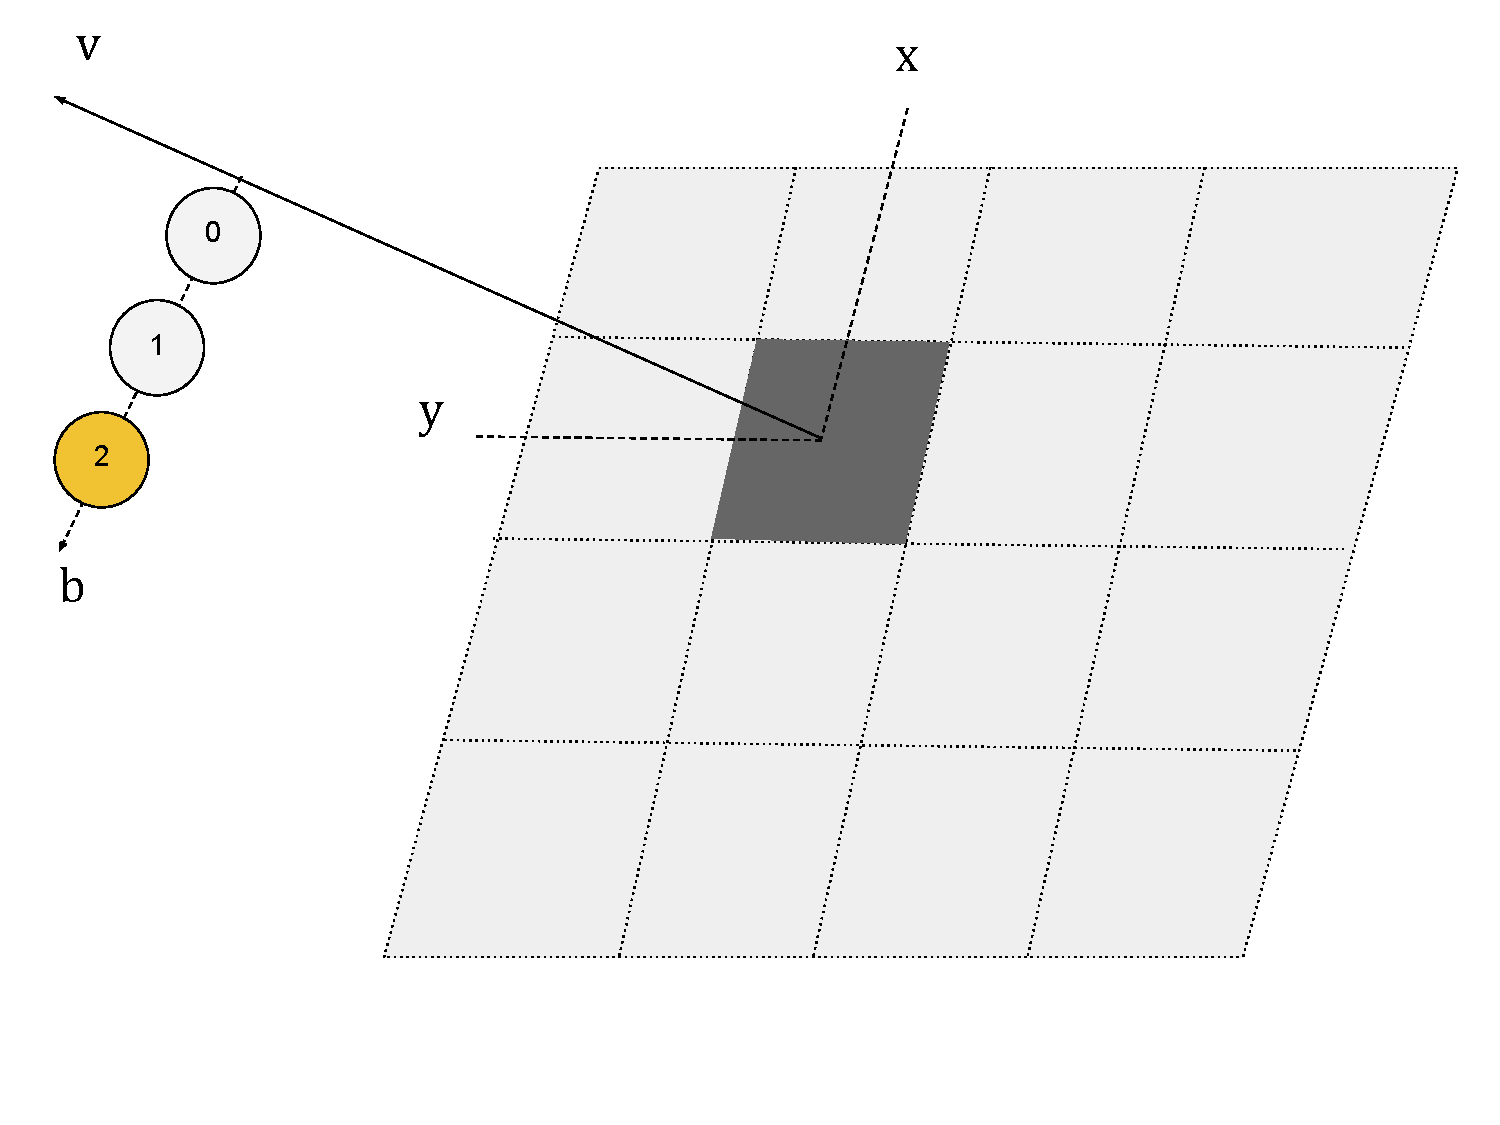
\includegraphics[scale=0.3]{fig/g003.pdf}
\end{figure}
\end{frame}

\begin{frame}[label=structures4]
\transdissolve[duration=1]
\frametitle{Graphe des états possibles}
\begin{figure}[!h]
\centering
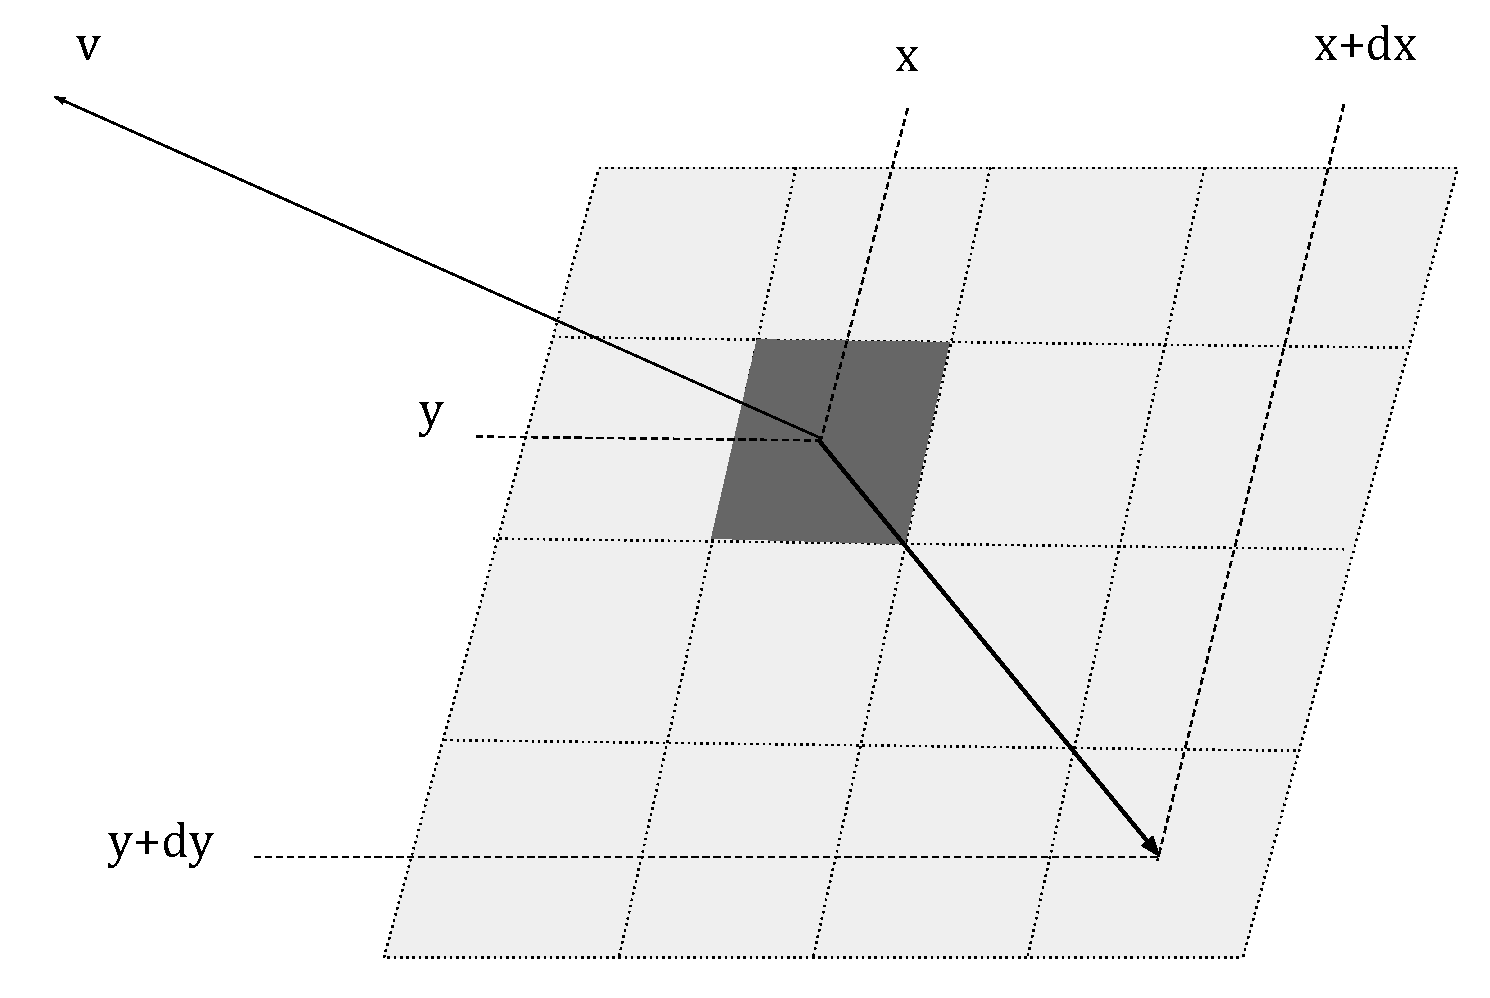
\includegraphics[scale=0.3]{fig/g004.pdf}
\end{figure}
\end{frame}

\begin{frame}[label=structures5]
\transdissolve[duration=1]
\frametitle{Graphe des états possibles}
\begin{figure}[!h]
\centering
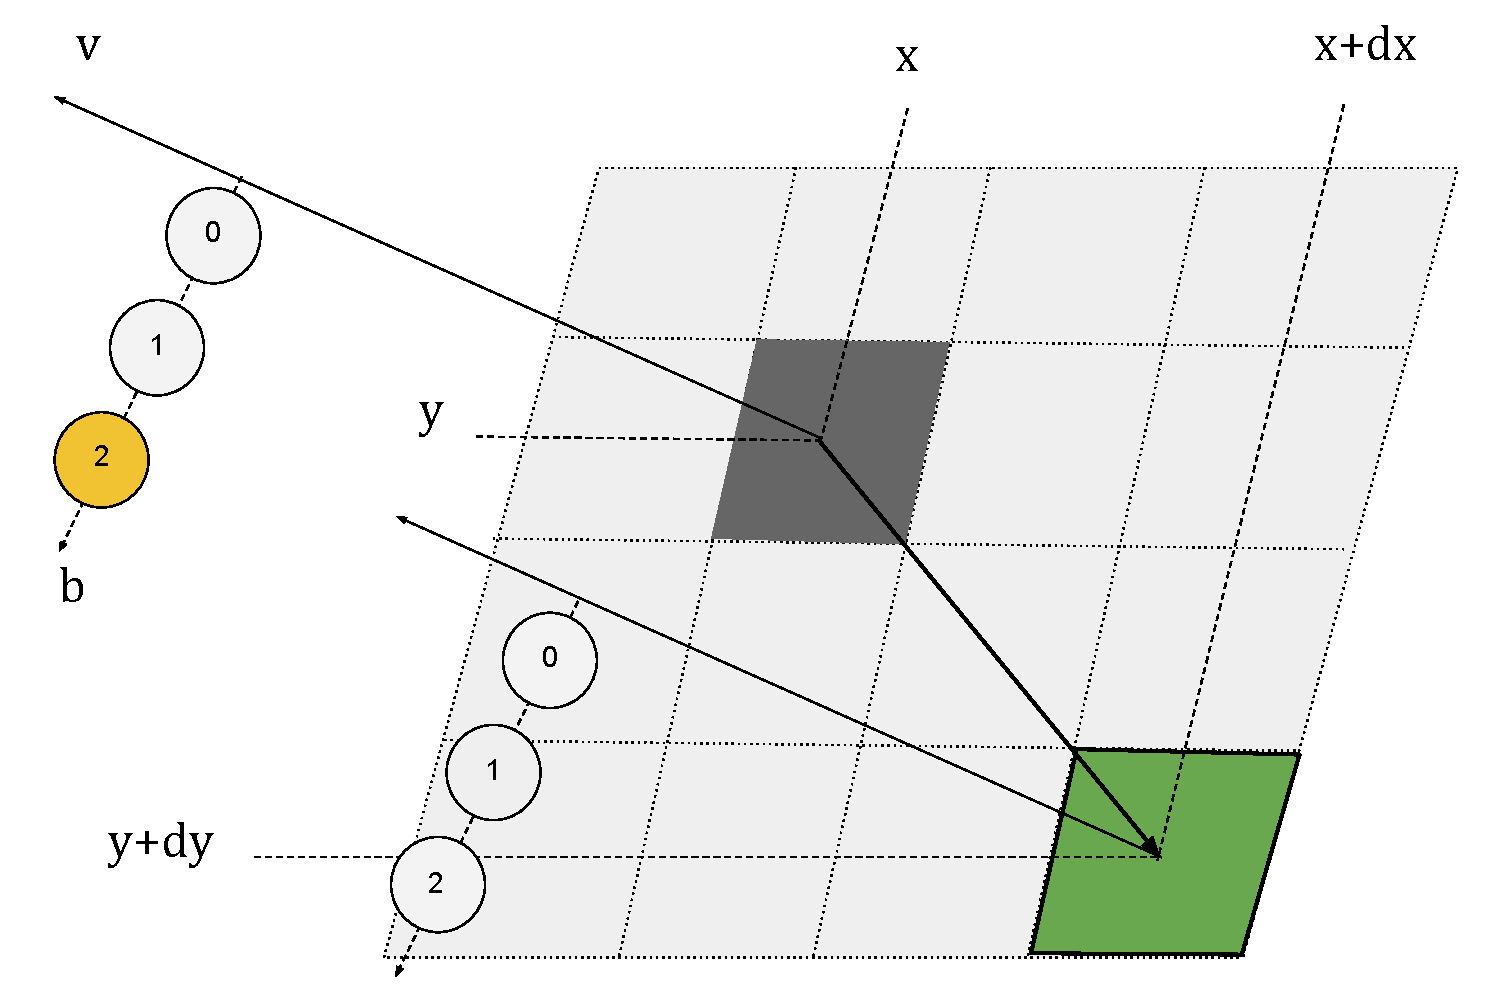
\includegraphics[scale=0.3]{fig/g005.pdf}
\end{figure}
\end{frame}

\begin{frame}[label=structures5]
\transdissolve[duration=1]
\frametitle{Graphe des états possibles}
\begin{figure}[!h]
\centering
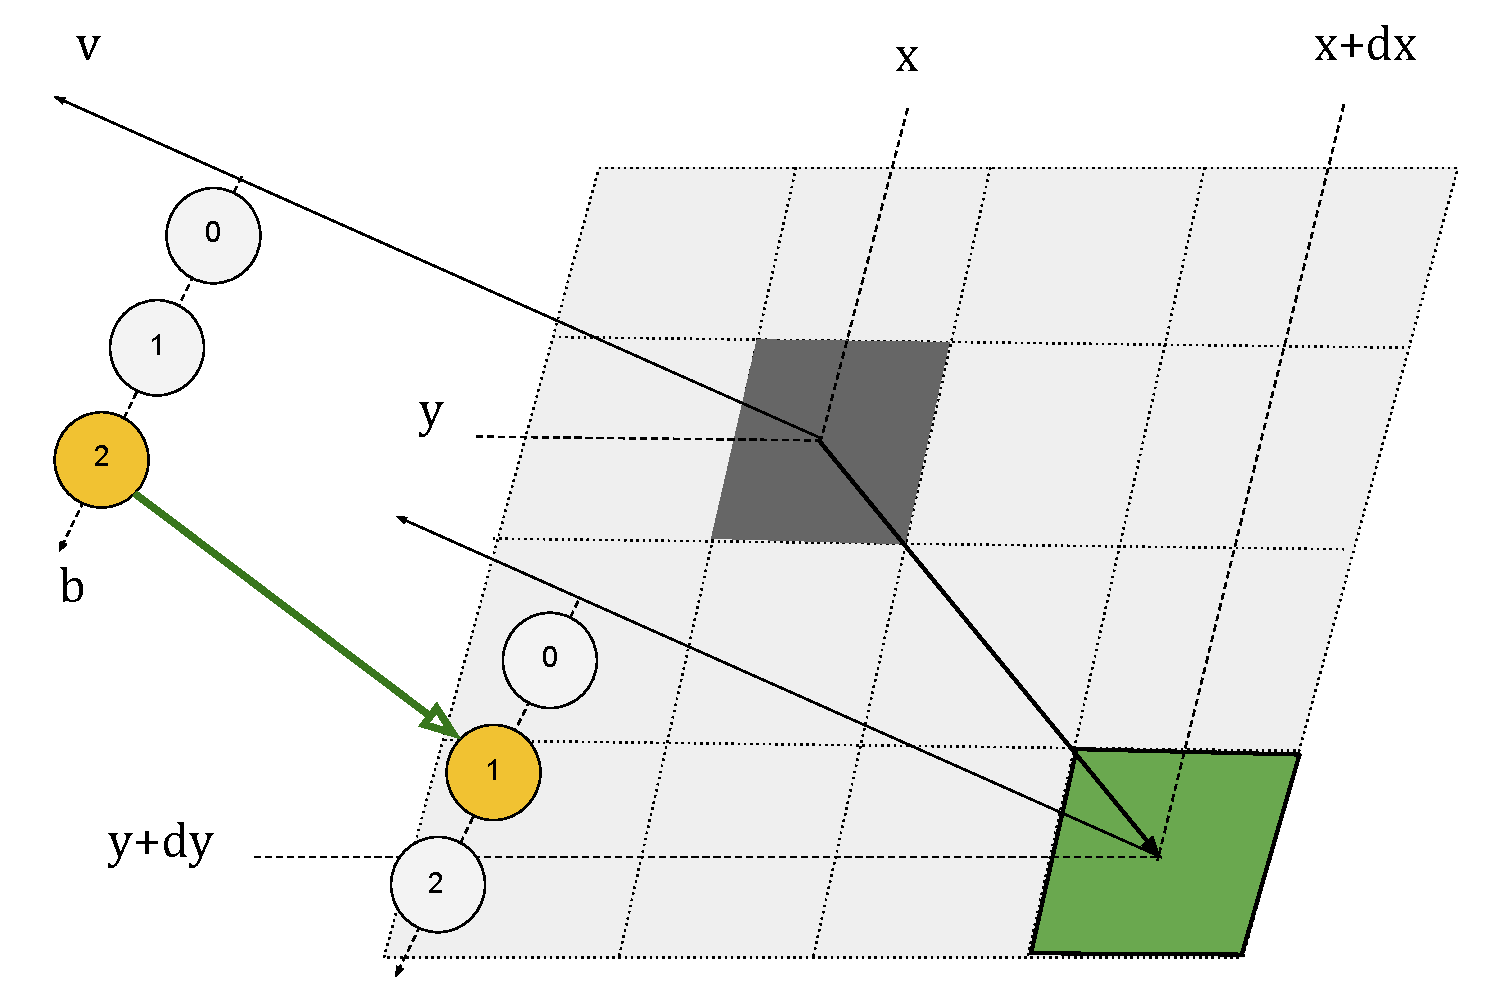
\includegraphics[scale=0.3]{fig/g006.pdf}
\end{figure}
\end{frame}

\begin{frame}[label=strategie]
\transdissolve[duration=1]
\frametitle{Stratégie de course}
\section{Stratégie de course}
Calcul du chemin optimal et mise à jour dynamique.
\end{frame}

\begin{frame}[label=strategie1]
\transdissolve[duration=1]
\frametitle{Stratégie de course}
\begin{figure}[!h]
\centering
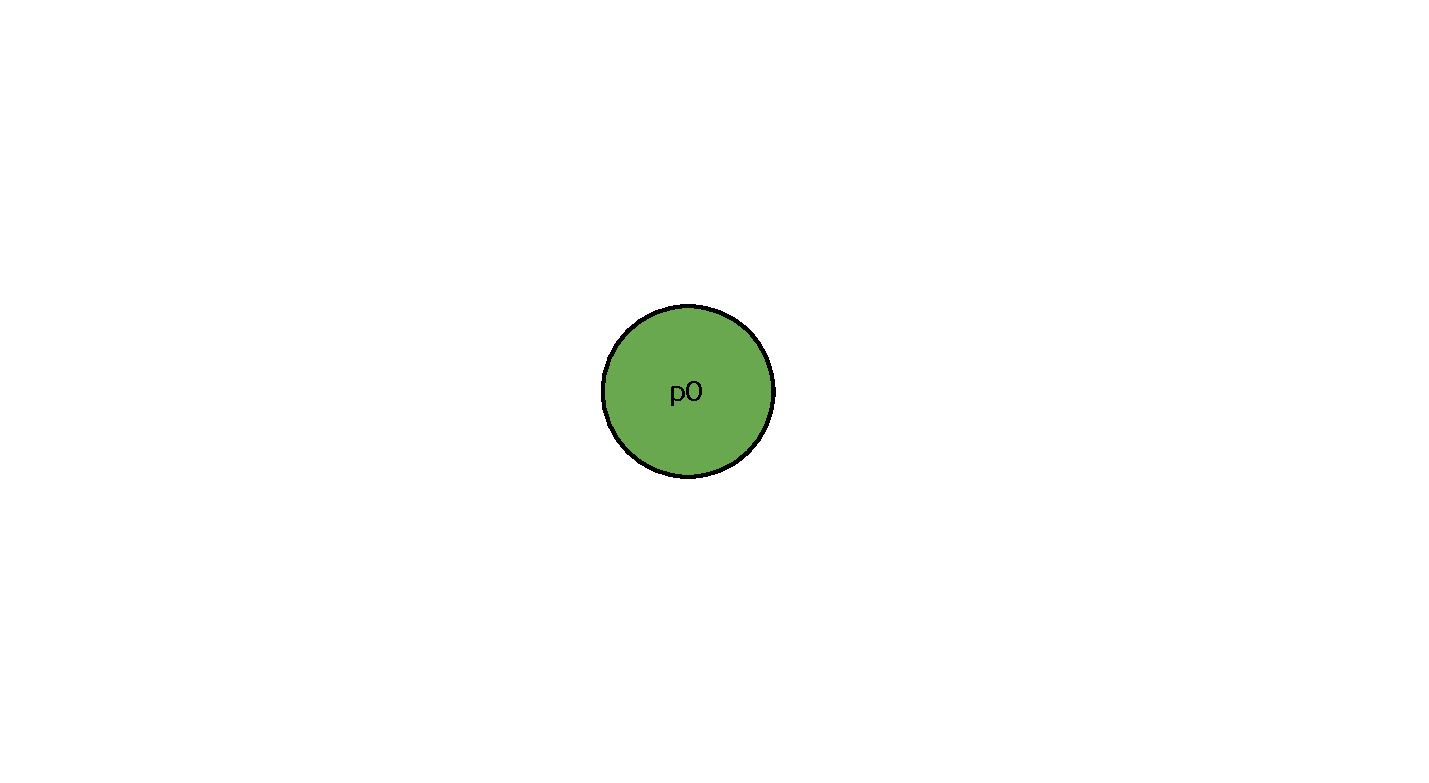
\includegraphics[scale=0.3]{fig/diag3.pdf}
\end{figure}
\end{frame}

\begin{frame}[label=strategie2]
\transdissolve[duration=1]
\frametitle{Stratégie de course}
\begin{figure}[!h]
\centering
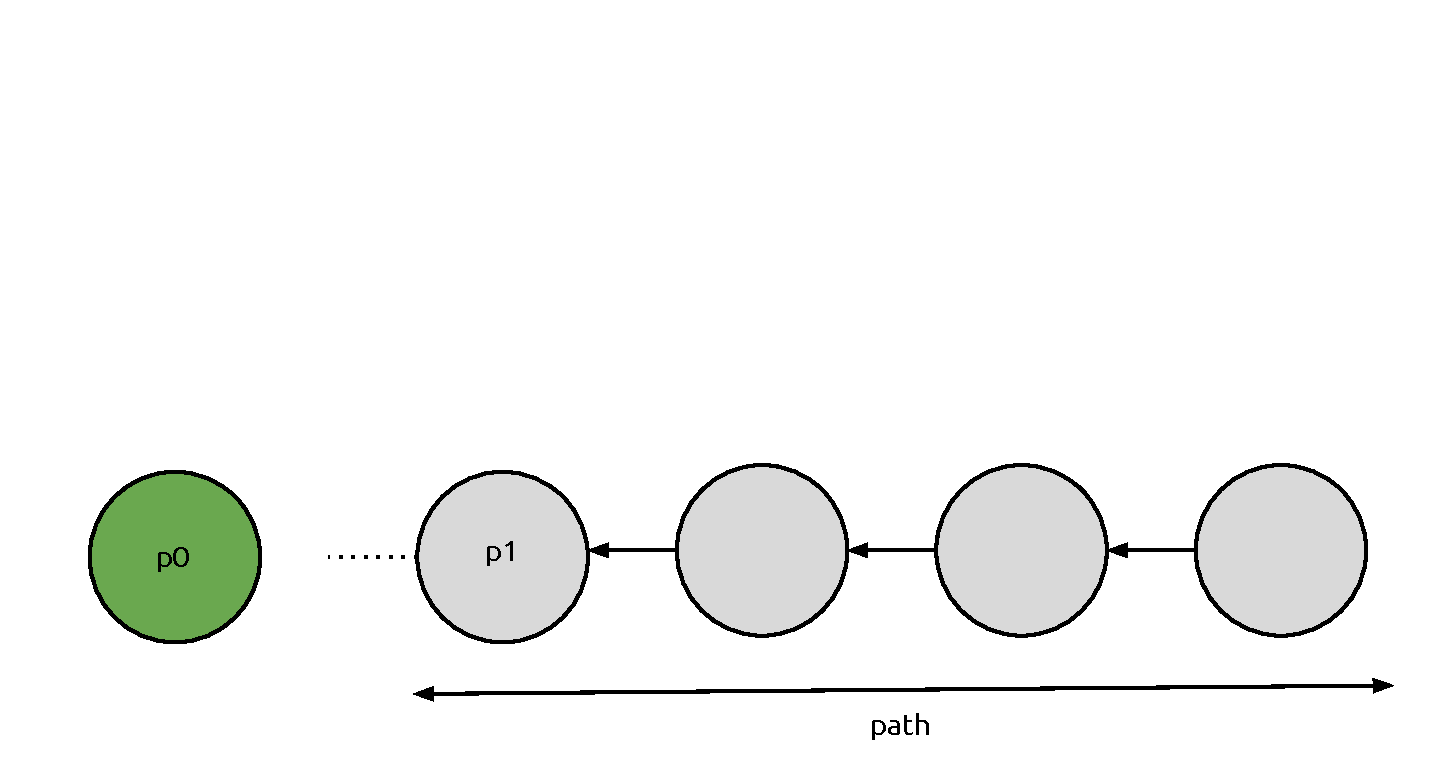
\includegraphics[scale=0.3]{fig/diag4.pdf}
\end{figure}
\end{frame}

\begin{frame}[label=strategie3]
\transdissolve[duration=1]
\frametitle{Stratégie de course}
\begin{figure}[!h]
\centering
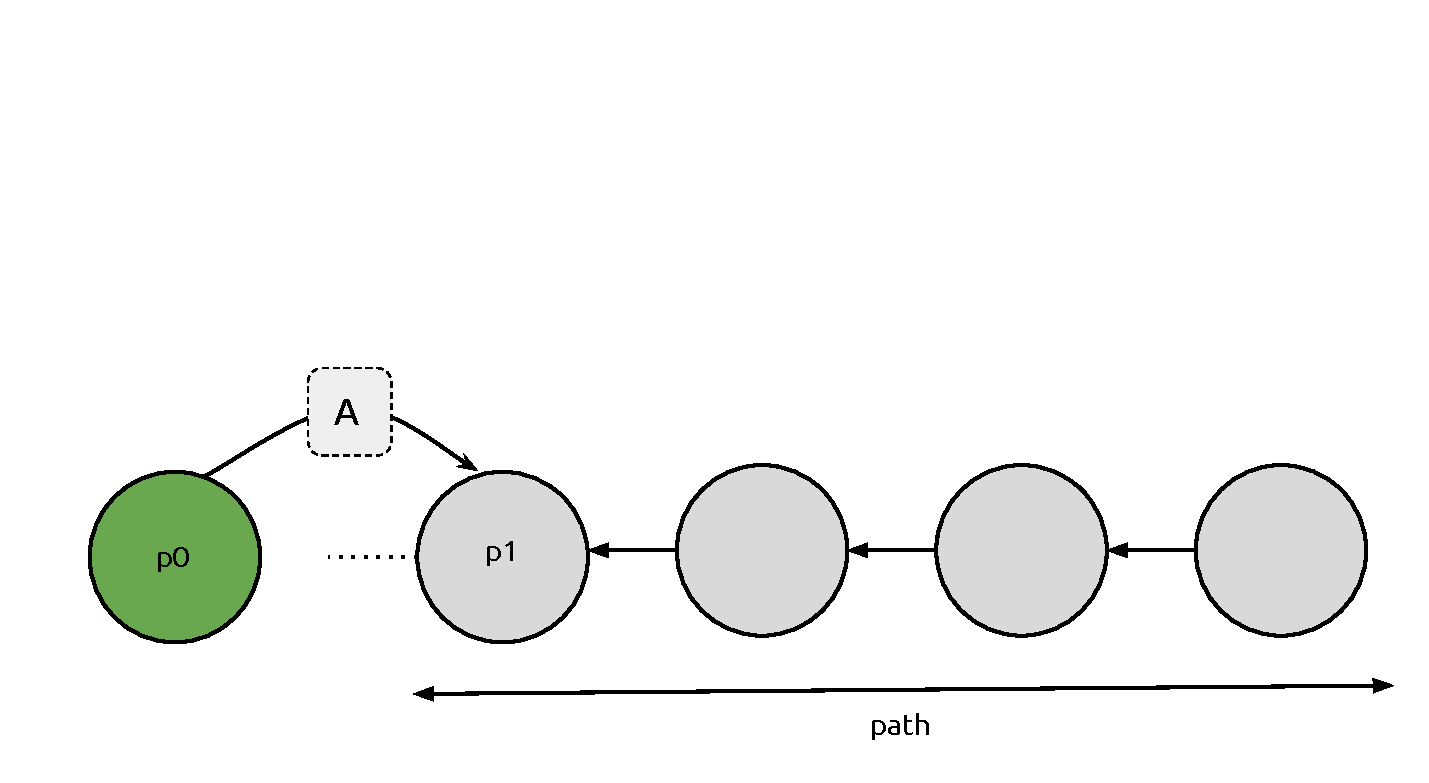
\includegraphics[scale=0.3]{fig/diag5.pdf}
\end{figure}
\end{frame}

\begin{frame}[label=strategie4]
\transdissolve[duration=1]
\frametitle{Stratégie de course}
\begin{figure}[!h]
\centering
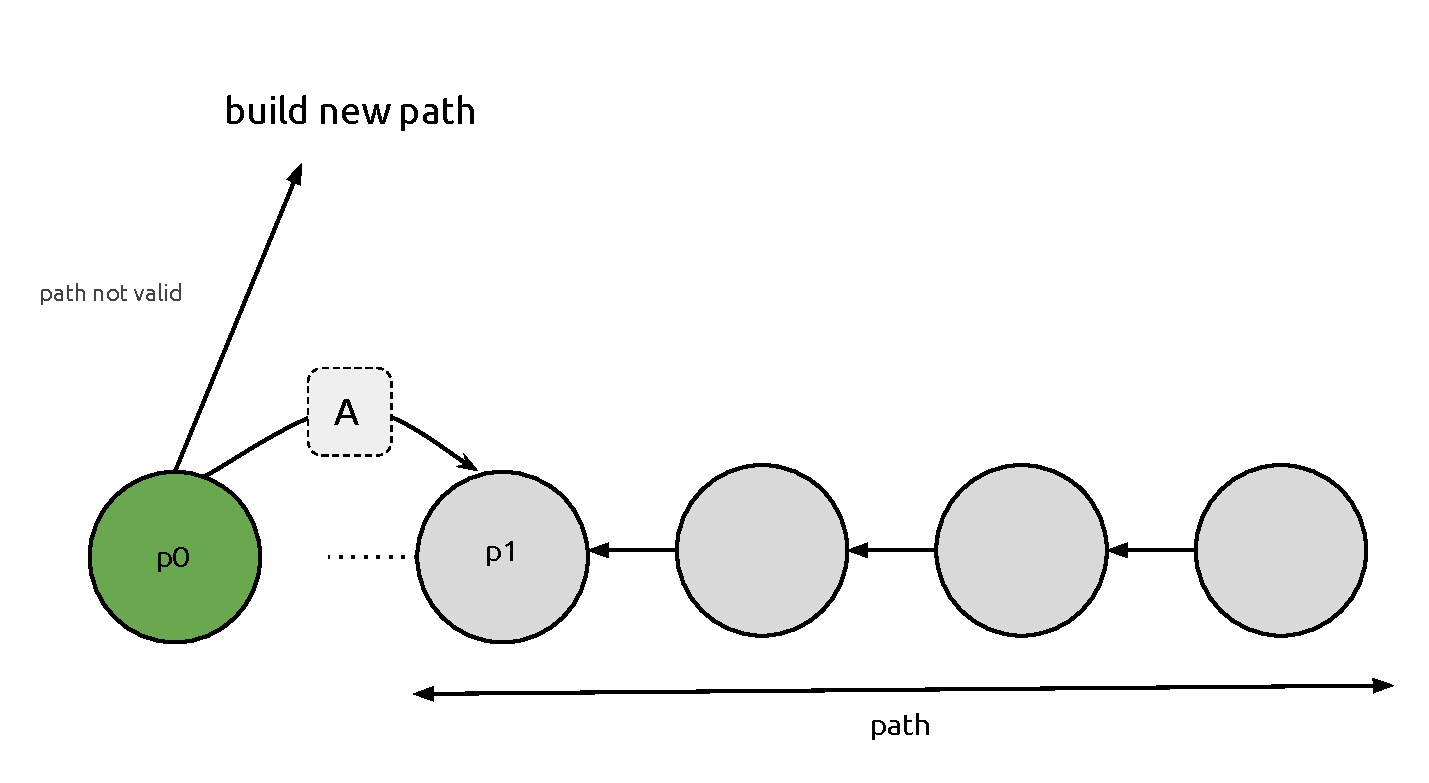
\includegraphics[scale=0.3]{fig/diag6.pdf}
\end{figure}
\end{frame}

\begin{frame}[label=strategie5]
\transdissolve[duration=1]
\frametitle{Stratégie de course}
\begin{figure}[!h]
\centering
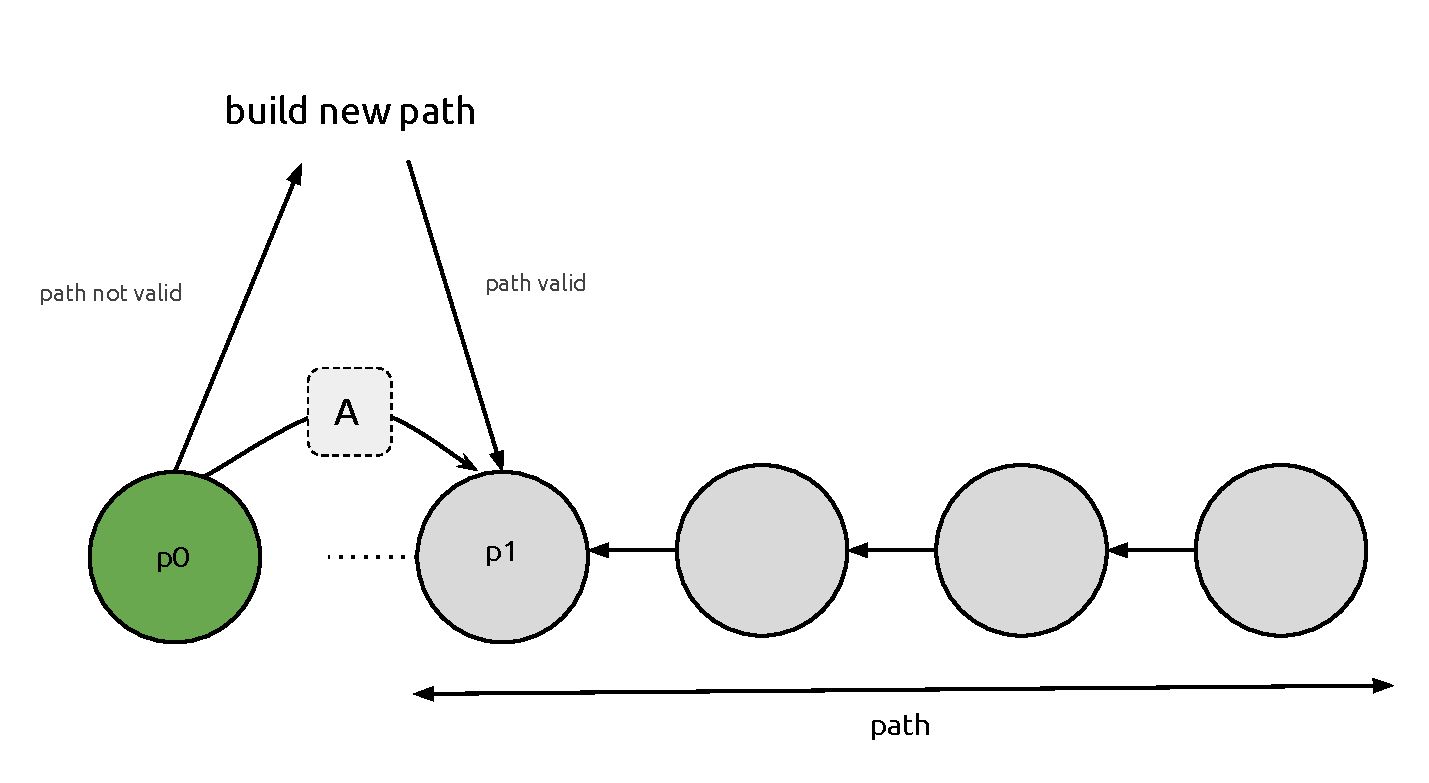
\includegraphics[scale=0.3]{fig/diag7.pdf}
\end{figure}
\end{frame}

\begin{frame}[label=strategie6]
\transdissolve[duration=1]
\frametitle{Stratégie de course}
\begin{figure}[!h]
\centering
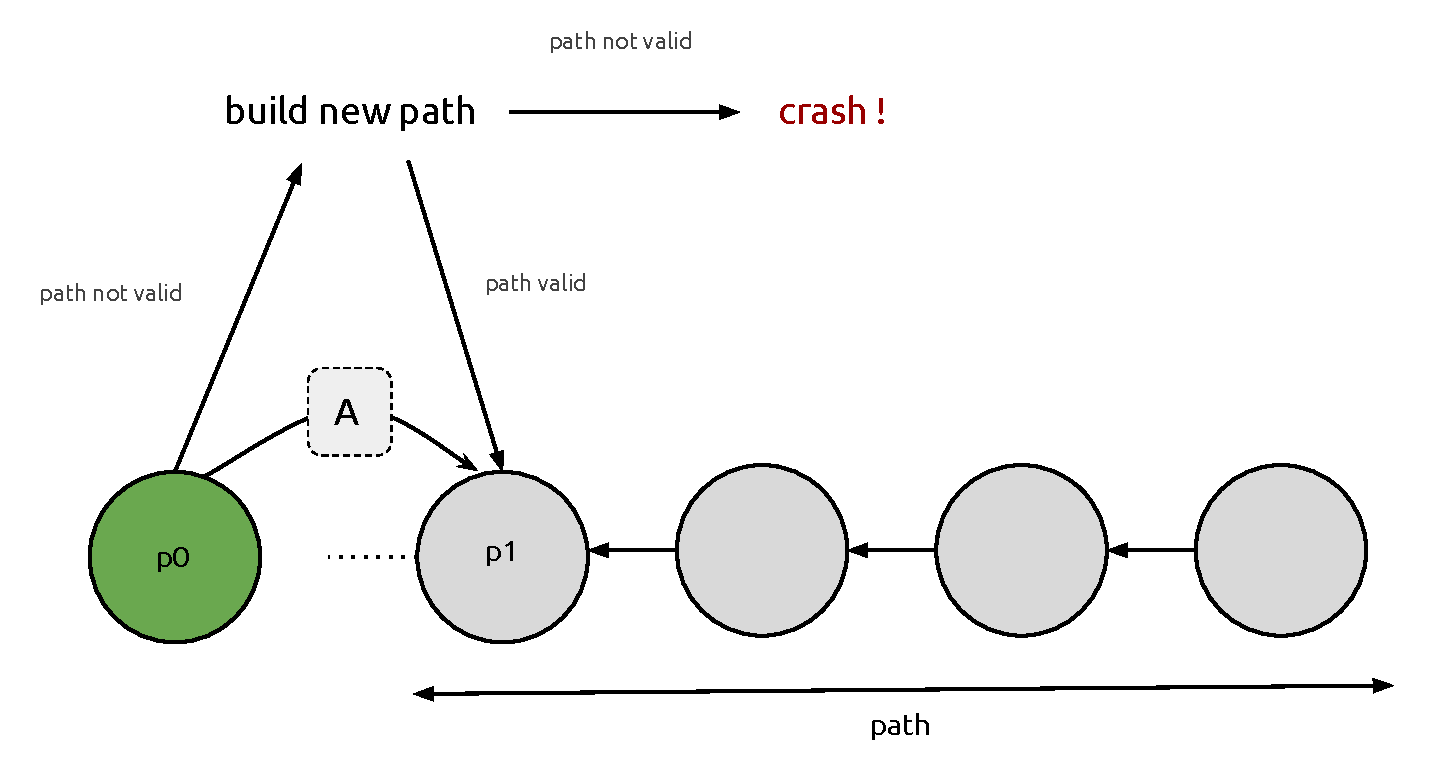
\includegraphics[scale=0.3]{fig/diag8.pdf}
\end{figure}
\end{frame}

\begin{frame}[label=strategie7]
\frametitle{Stratégie de course}
\begin{figure}[!h]
\centering
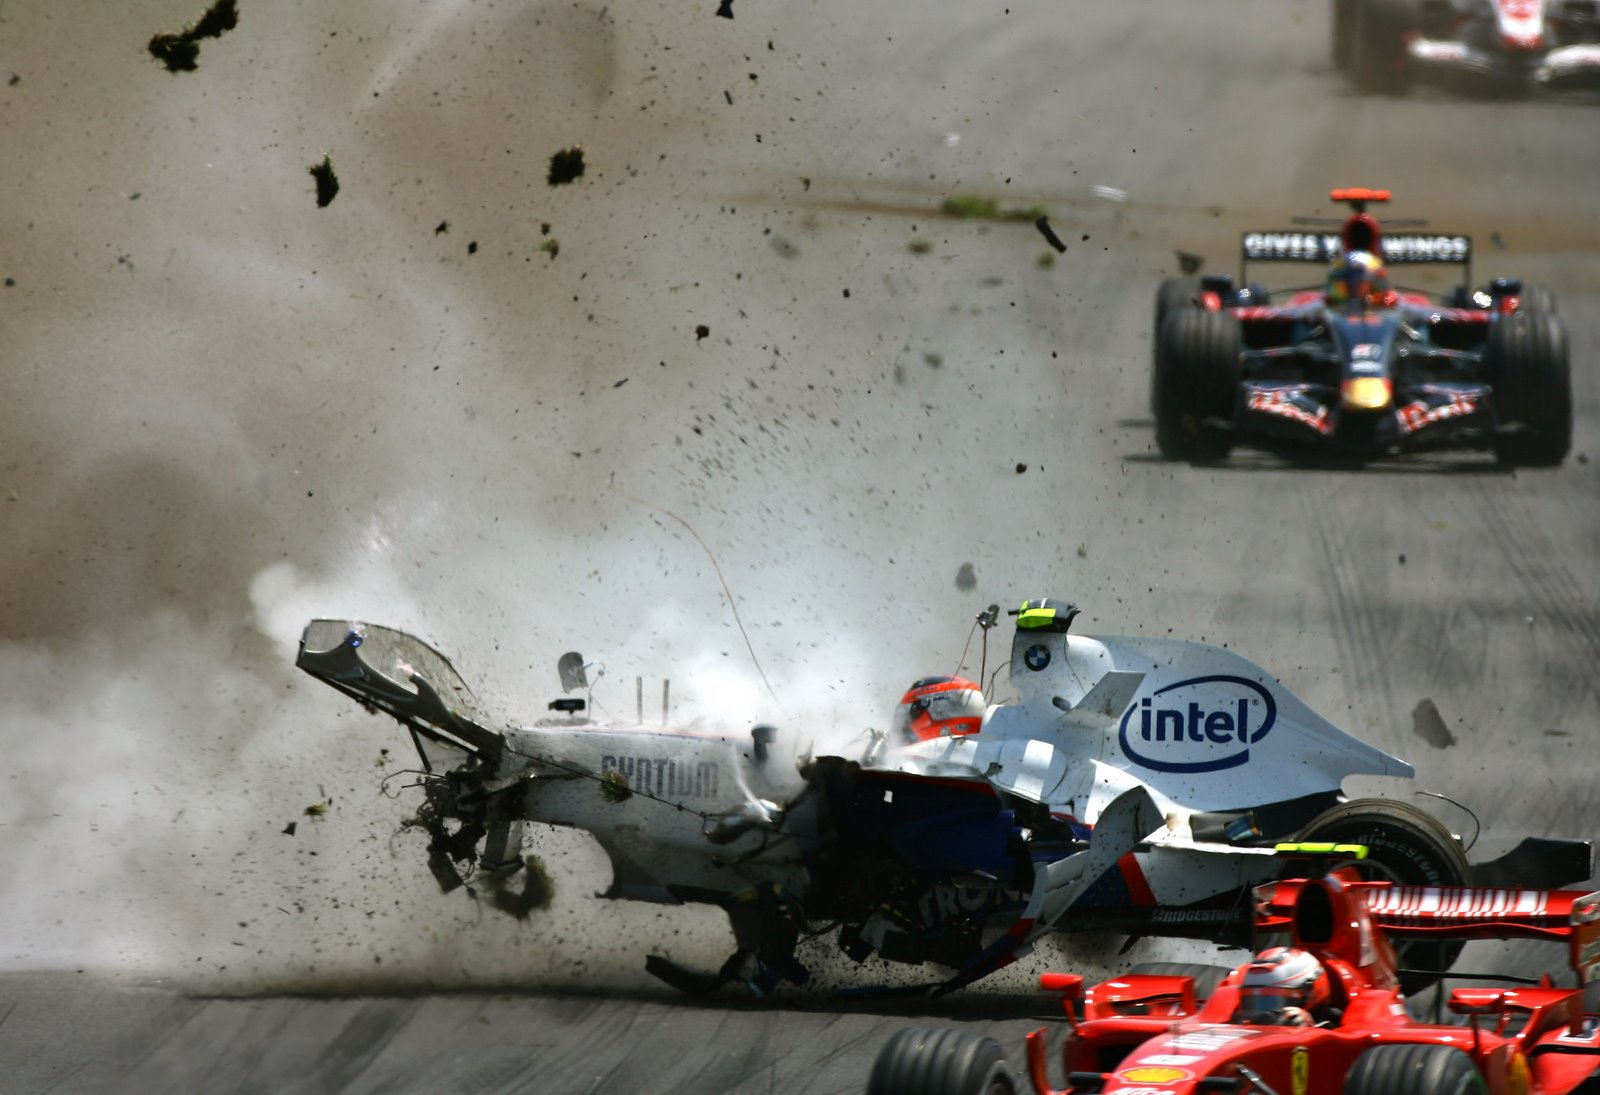
\includegraphics[scale=0.18]{fig/crash.jpg}
\end{figure}
\end{frame}

\begin{frame}[label=resultats]
\transdissolve[duration=1]
\frametitle{Quelques résultats}
\begin{tabular}{|c|c|c|c|}
  \hline
  Carte/Pilote& GPDriverOne & GPDriverTwo & Mon pilote \\
  \hline
  Droit au but &13 & 9 & 6 \\
  Virages &112 & 75 & 39 \\
  Virages et sable & 430 & 354& 41\\
  Serpent & 257 & 77& 33\\
  \hline
\end{tabular}
\end{frame}

\end{document}
